\chapter{Cyber Intelligence Visualization}

Objetivo principal: producir para analistas y responsables de la toma de decisiones mecanismos útiles para
comprender, de un vistazo, la información relevante y las tendencias dentro de las enormes cantidades
de datos en bruto que les proporcionamos actualmente en las herramientas cibernéticas.

Las herramientas  de ciber inteligencia generan una gran cantidad de datos, en gran parte testuale, y es necesario que los analistas sean capaces de procesarlos y entenderlos de manera rápida y eficiente.

Es frequentemente necesario representar multi-dimensional data en un espacio 2D o 3D.

Los puntos clave de la visualización de la inteligencia cibernética son:
\begin{itemize}
   \item Dimensionality reduction and complexity reduction.
   \item Assuming inhernet non-linearities and couplings
   \item Tools and visualization techniques are need to help in the iterative process:
   
\end{itemize}

\section{Visualization Charts}
\begin{table}[htbp]
   \centering
   \begin{tabular}{|c|c|c|c|c|}
\hline Area     & Bar       & BoxPlot      & Bubble       & Column \\
\hline Doughnut & ErrorBar  & FastLine     & Funnel       & Kagi \\
\hline Line     & Pie       & Point        & Polar        & Radar \\
\hline Range    & Spline    & StackedArea  & StackedBar   & StepLine\\
\hline
   \end{tabular}
   \caption{Basic tecniques for Cyber Intelligence Visualization}
   \label{tab:03/tecnicasVisualizacion}
\end{table}

\begin{paracol}{2}
   
   Los investigadores y profesionales descubrieron que las técnicas de visualización existentes no satisfacen las necesidades de representación del ciberespacio, mientras que la \emph{graph-based} visualización gráficos proporciona medios para mostrar datos interrelacionados multidimensionales en un gráfico de pocas dimensiones.\\
   Una tecnica eficiente para reducir las dimensiones de los datos es utilizar el color.

   \switchcolumn
   \begin{figure}[htbp]
      \centering
      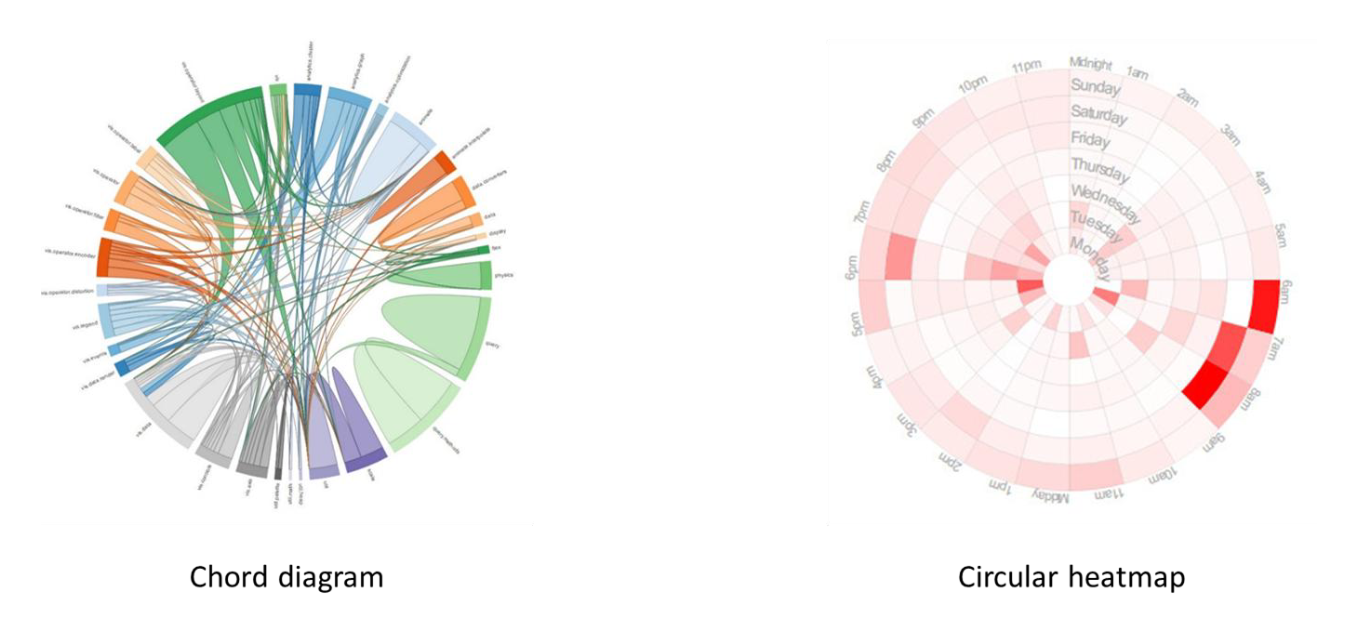
\includegraphics{images/03/color.png}
      \caption{Relational color-based dimension reduction}
      \label{fig:03/color}
   \end{figure}
\end{paracol}

\begin{figure}[htbp]
   \centering
   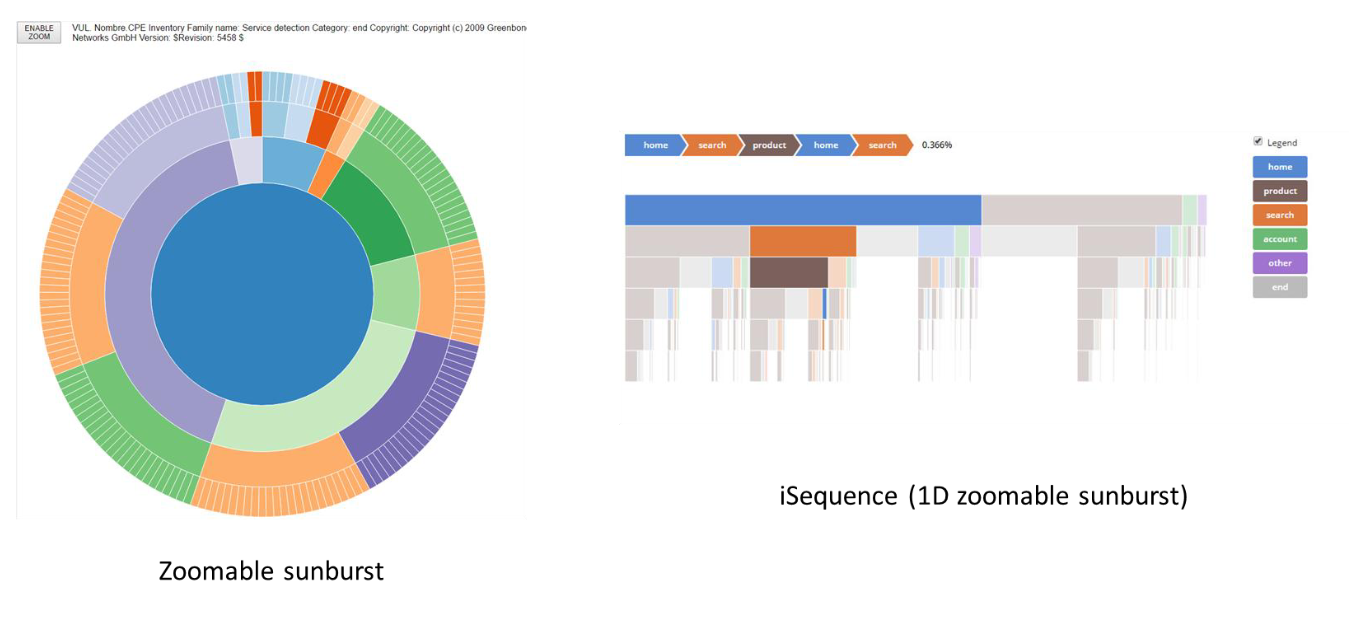
\includegraphics{images/03/sunburst.png}
   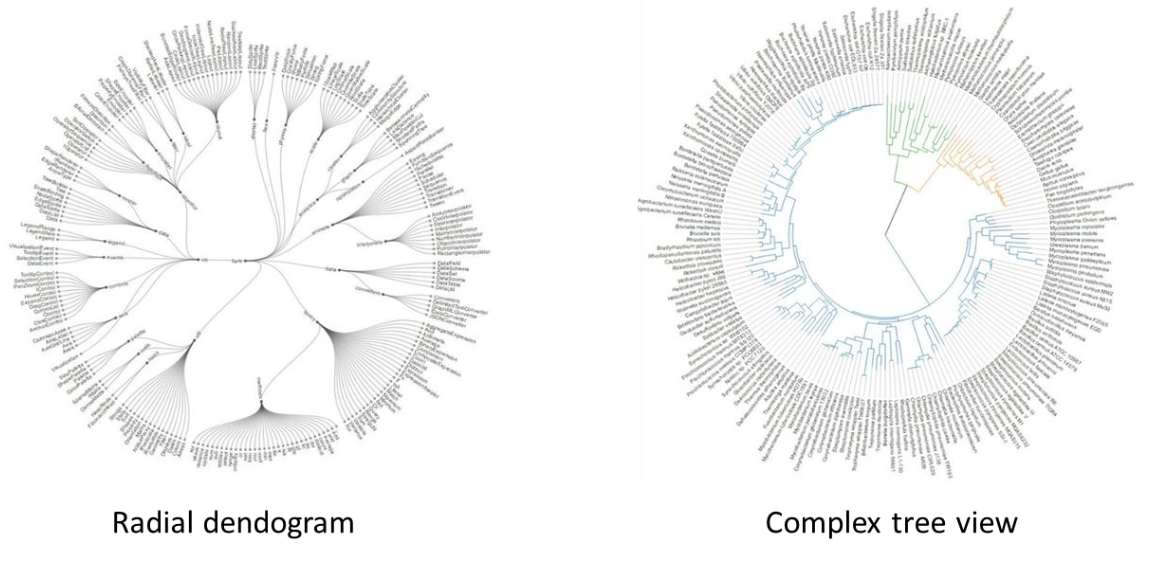
\includegraphics{images/03/dendogram.png}
   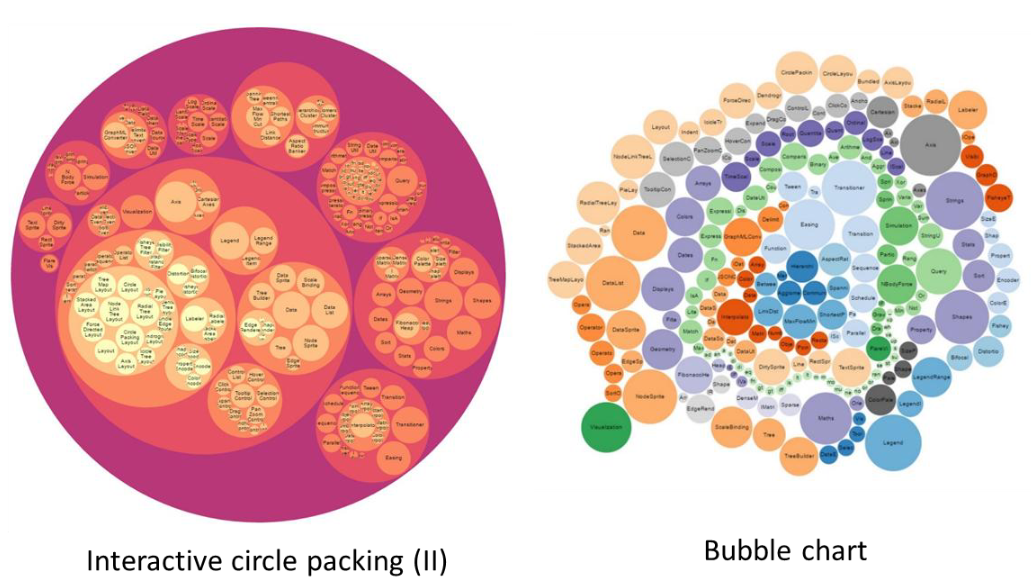
\includegraphics{images/03/circlepacking.png}
   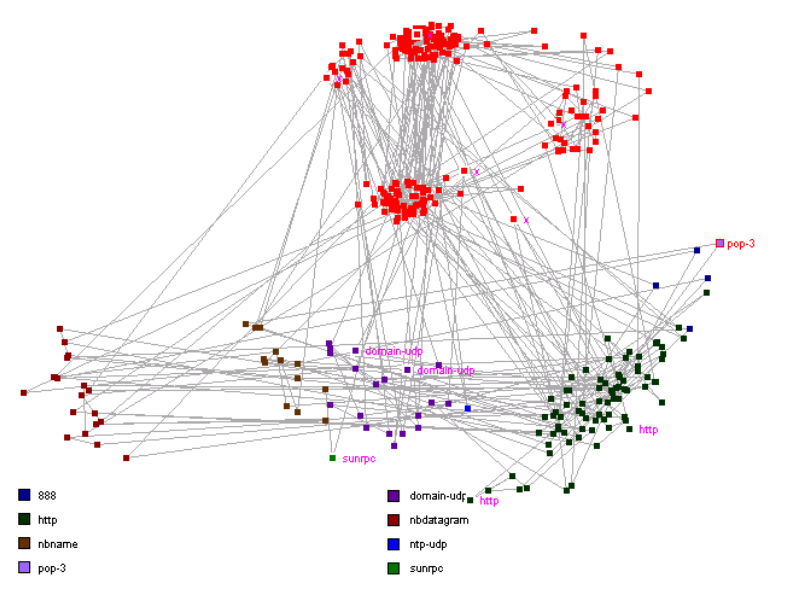
\includegraphics{images/03/interactivenodelinks.png}
   \caption{Graph-based visualización techniques}
   \label{fig:03/graphbased}
\end{figure}

\begin{figure}[htbp]
   \centering
   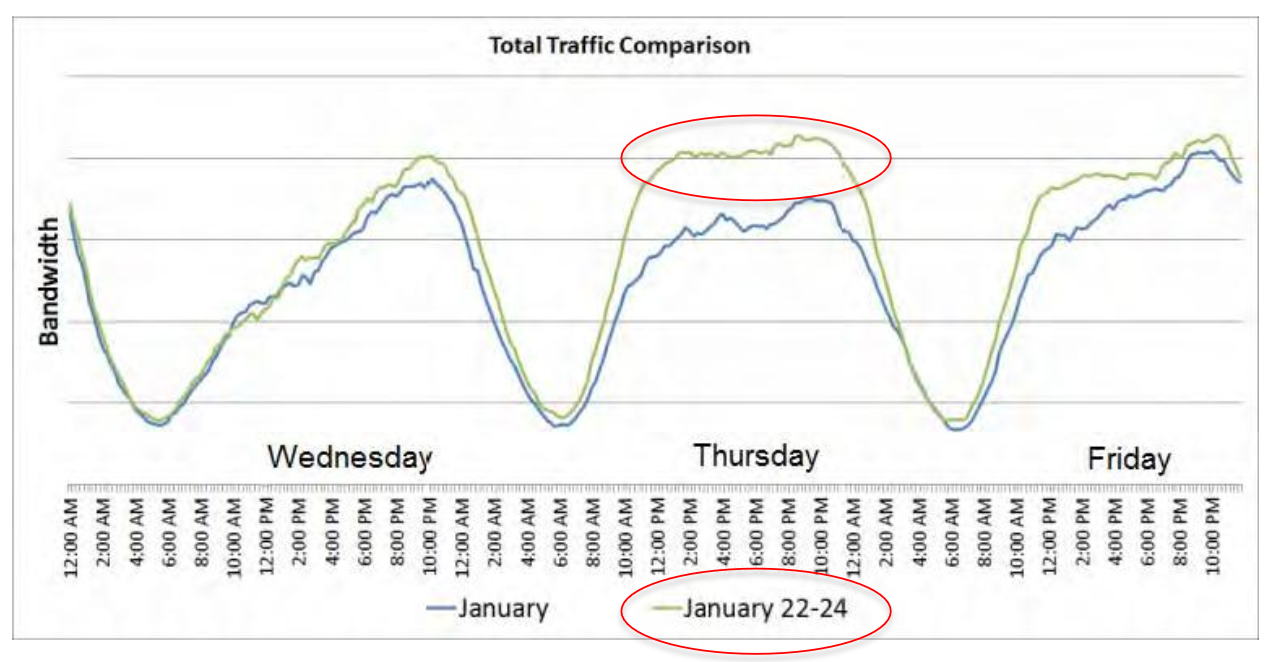
\includegraphics{images/03/ddos.png}
   \caption{Según el profesor, este gráfico es muy importante porque muestra que para identificar lo que es \emph{anormal}, es necesario saber lo que es \emph{normal}.}
   \label{fig:03/ddos}
\end{figure}